\begin{frame}{Testing Data Distribution Analysis}

    \begin{columns}

        % Left Column: Explanation
        \column{0.50\textwidth}
        \textbf{Why Ensure Balanced Testing Data?}
        \begin{itemize}
     \item Prevents bias toward majority classes.
        \item Ensures the model's performance is fairly evaluated.
        \item Helps achieve reliable generalization across all sleep stages.
           \item The figure shows the normalized class distribution during testing.
        \item Each class maintains an equalized density, avoiding class imbalance.
        \item This confirms that the model's evaluation is not biased toward any specific sleep stage.
        \end{itemize}

        % Right Column: Sampling Density Plot
        \column{0.50\textwidth}
        \centering
        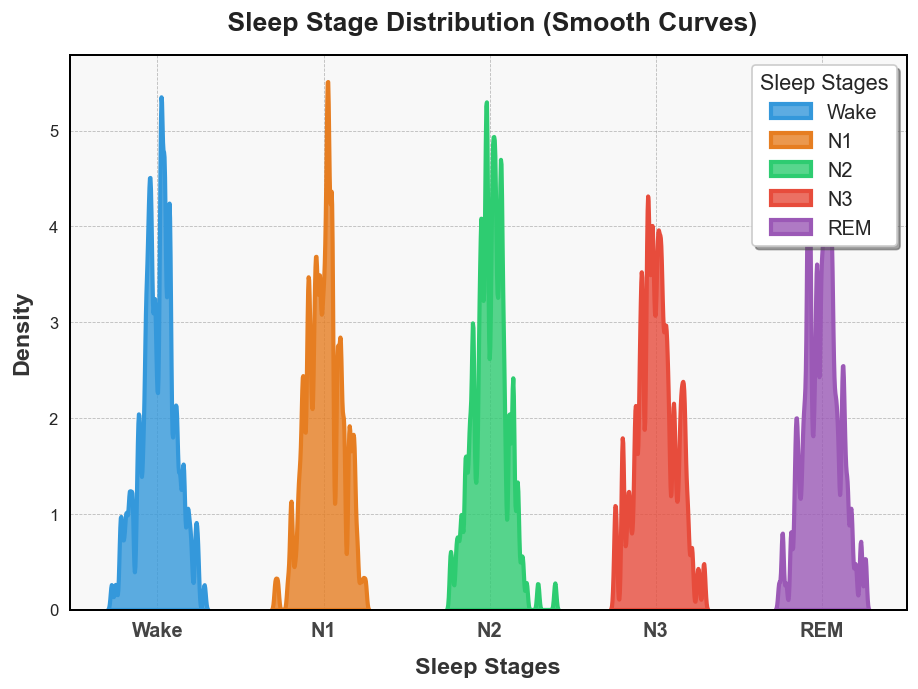
\includegraphics[width=0.9\linewidth]{images/paper_3/sample distribution plot pdf.png} % Replace with actual figure
        \vspace{5pt}
        {\textcolor{uwopurple}{\small Sampling Density Plot Showing Balanced Class Distribution}}

    \end{columns}

\end{frame}


\begin{frame}{Model Performance: Training vs Testing}

    \begin{columns}

        % Left Column: Accuracy Plot
        \column{0.50\textwidth}
        \centering
        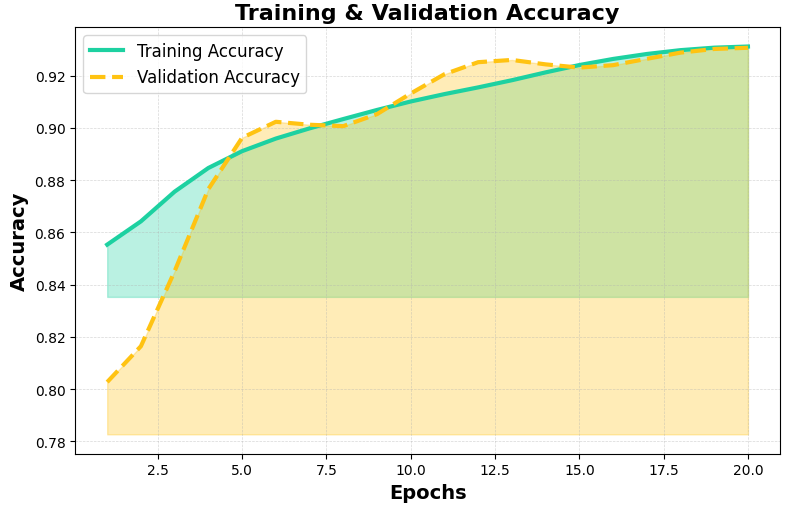
\includegraphics[width=1\linewidth]{images/paper_3/accuracy plot.png} % Replace with actual file
        \captionof{figure}{\textcolor{uwopurple}{ Accuracy Curve}}

        % Right Column: Loss Plot
        \column{0.50\textwidth}
        \centering
        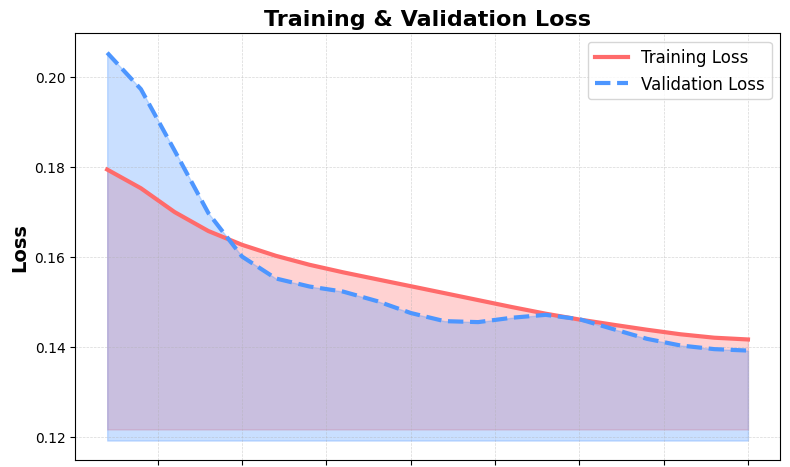
\includegraphics[width=1\linewidth]{images/paper_3/loss plot.png} % Replace with actual file
        \captionof{figure}{\textcolor{uwopurple}{ Loss Curve}}

    \end{columns}

\end{frame}



\begin{frame}{Model Evaluation: Confusion Matrix}

    \begin{columns}

        % Left Column: Precision, Recall, F1-Score Formulas
        \column{0.50\textwidth}
        \textbf{Performance Metrics}
        \vspace{10pt}
        
        \textbf{Precision:} 
        \[
        \text{Precision} = \frac{TP}{TP + FP}
        \]
        
        \textbf{Recall:} 
        \[
        \text{Recall} = \frac{TP}{TP + FN}
        \]

        \textbf{F1-Score:}
        \[
        \text{F1-Score} = \frac{2 \times \text{Precision} \times \text{Recall}}{\text{Precision} + \text{Recall}}
        \]

        \vspace{5pt}
        These metrics ensure a balanced evaluation of model performance across all classes.

        % Right Column: Confusion Matrix Plot
        \column{0.50\textwidth}
        \centering
        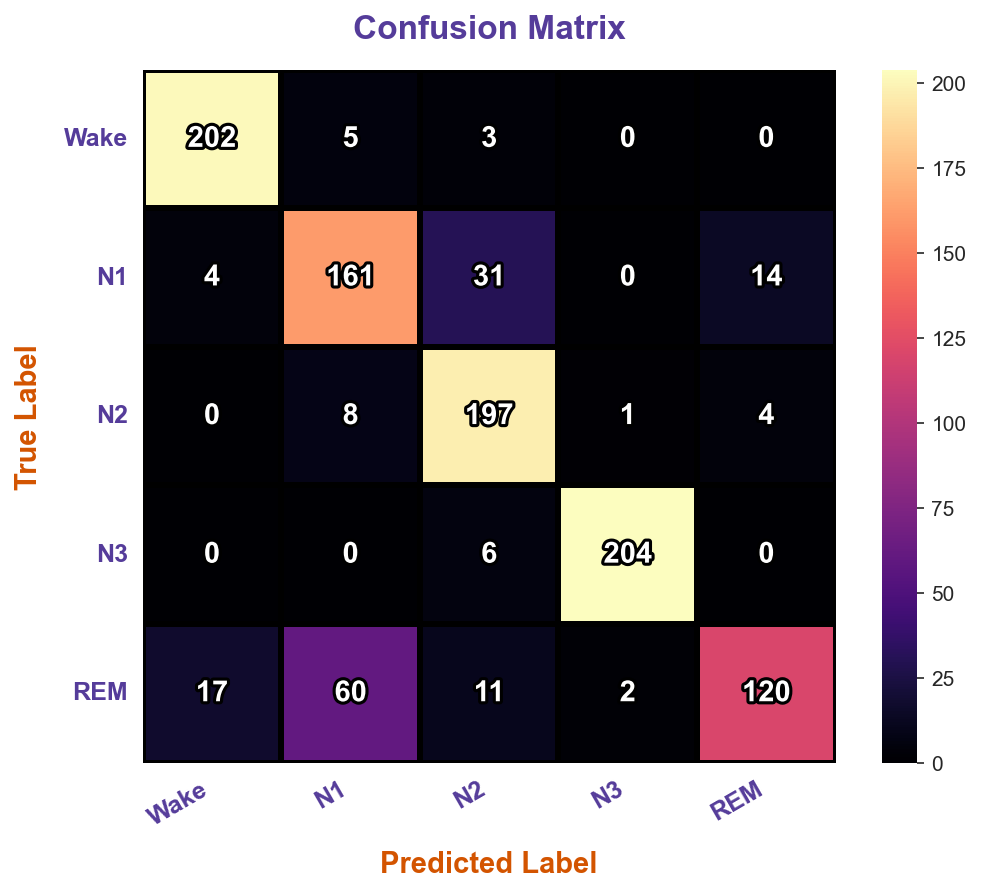
\includegraphics[width=0.9\linewidth]{images/paper_3/confusion matrix samples.png} % Replace with actual file
        \captionof{figure}{\textcolor{uwopurple}{Confusion Matrix }}

    \end{columns}

\end{frame}




\begin{frame}{Gradient Analysis: Training Progression}

    \begin{columns}

        % Left Column: Explanation of Training Behavior
        \column{0.50\textwidth}
        \textbf{Understanding Model Training Dynamics}
        \vspace{10pt}

      \begin{itemize}
            \item \textbf{Early Training (Epochs 0-5):} High loss, accuracy starts improving.
            \item \textbf{Mid Training (Epochs 5-15):} Loss steadily decreases, stable gradient flow.
            \item \textbf{Late Training (Epochs 15-20):} Accuracy plateaus, no severe overfitting.
        \end{itemize}

          \textbf{Conclusion:} The training process remains stable, with no vanishing or exploding gradients. 


        % Right Column: 3D Gradient Plot
        \column{0.50\textwidth}
        \centering
        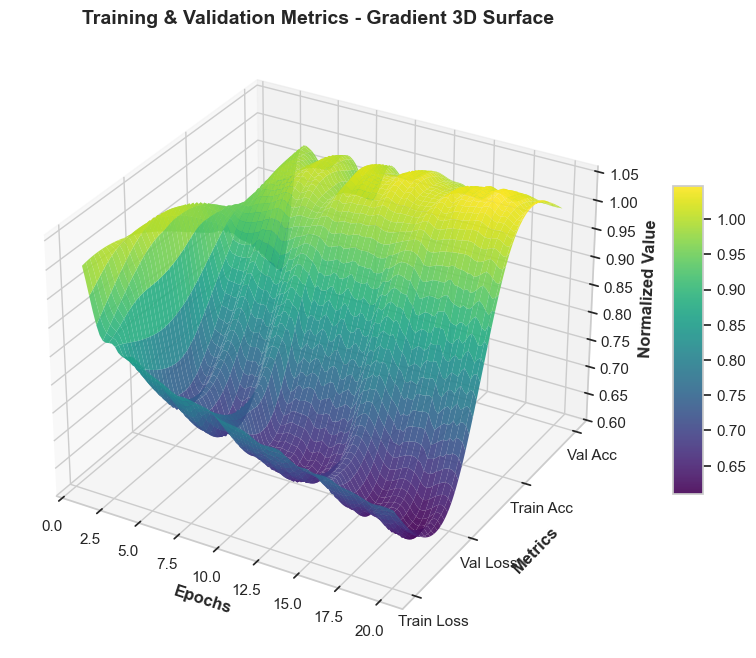
\includegraphics[width=0.9\linewidth]{images/paper_3/3d gradient.png} % Replace with actual file
        \captionof{figure}{\textcolor{purple}{Gradient 3D Surface: Training vs Validation Metrics}}

    \end{columns}

\end{frame}





\begin{frame}{Performance Metrics: Precision, Recall, F1-Score}

    \centering
    \textbf{Evaluating model performance across all classes using key metrics.}
    
    \vspace{10pt} % Add some space

    \begin{columns}
        % Left Column: Precision Bar Plot
        \column{0.33\textwidth}
        \centering
        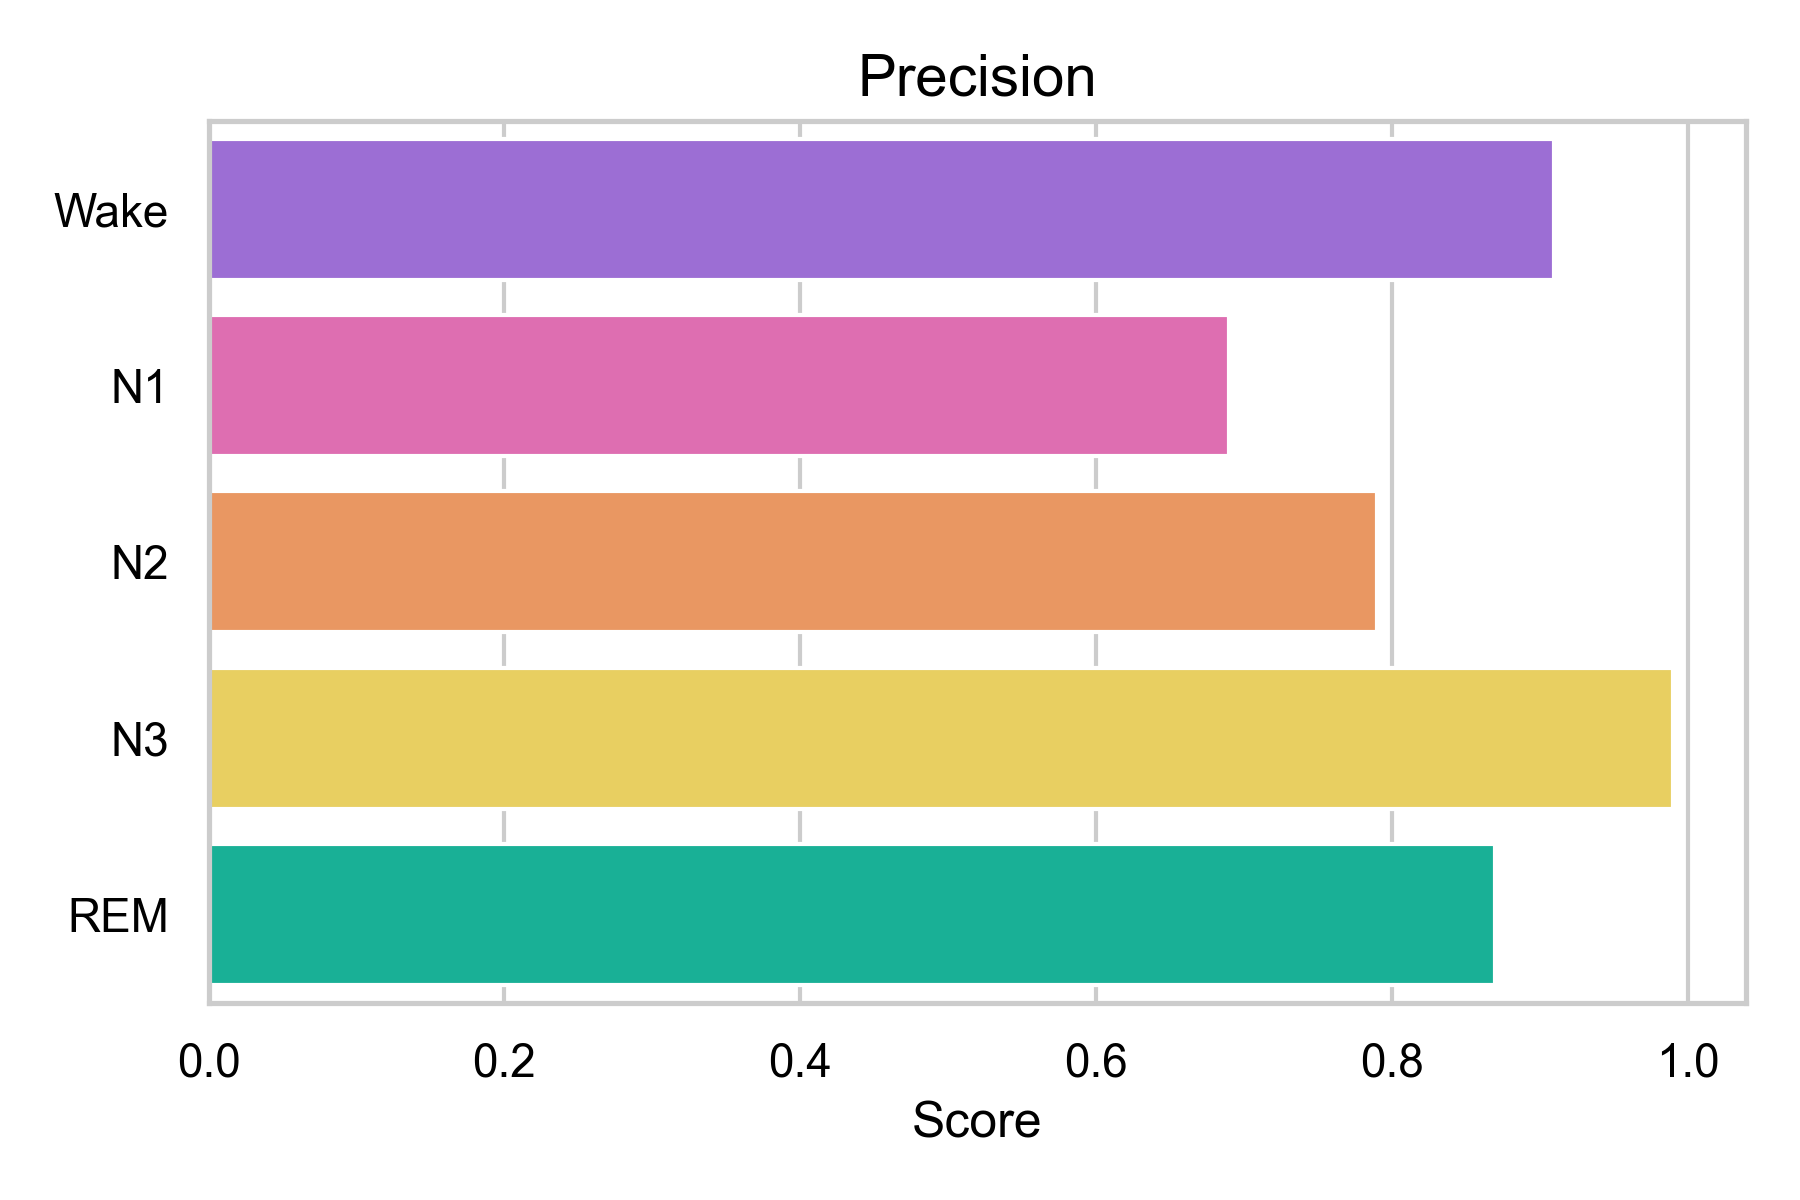
\includegraphics[width=\linewidth]{images/paper_3/precision_plot.png} % Replace with actual figure
        \captionof{figure}{\textcolor{purple}{Precision Scores per Class}}

        % Middle Column: Recall Bar Plot
        \column{0.33\textwidth}
        \centering
        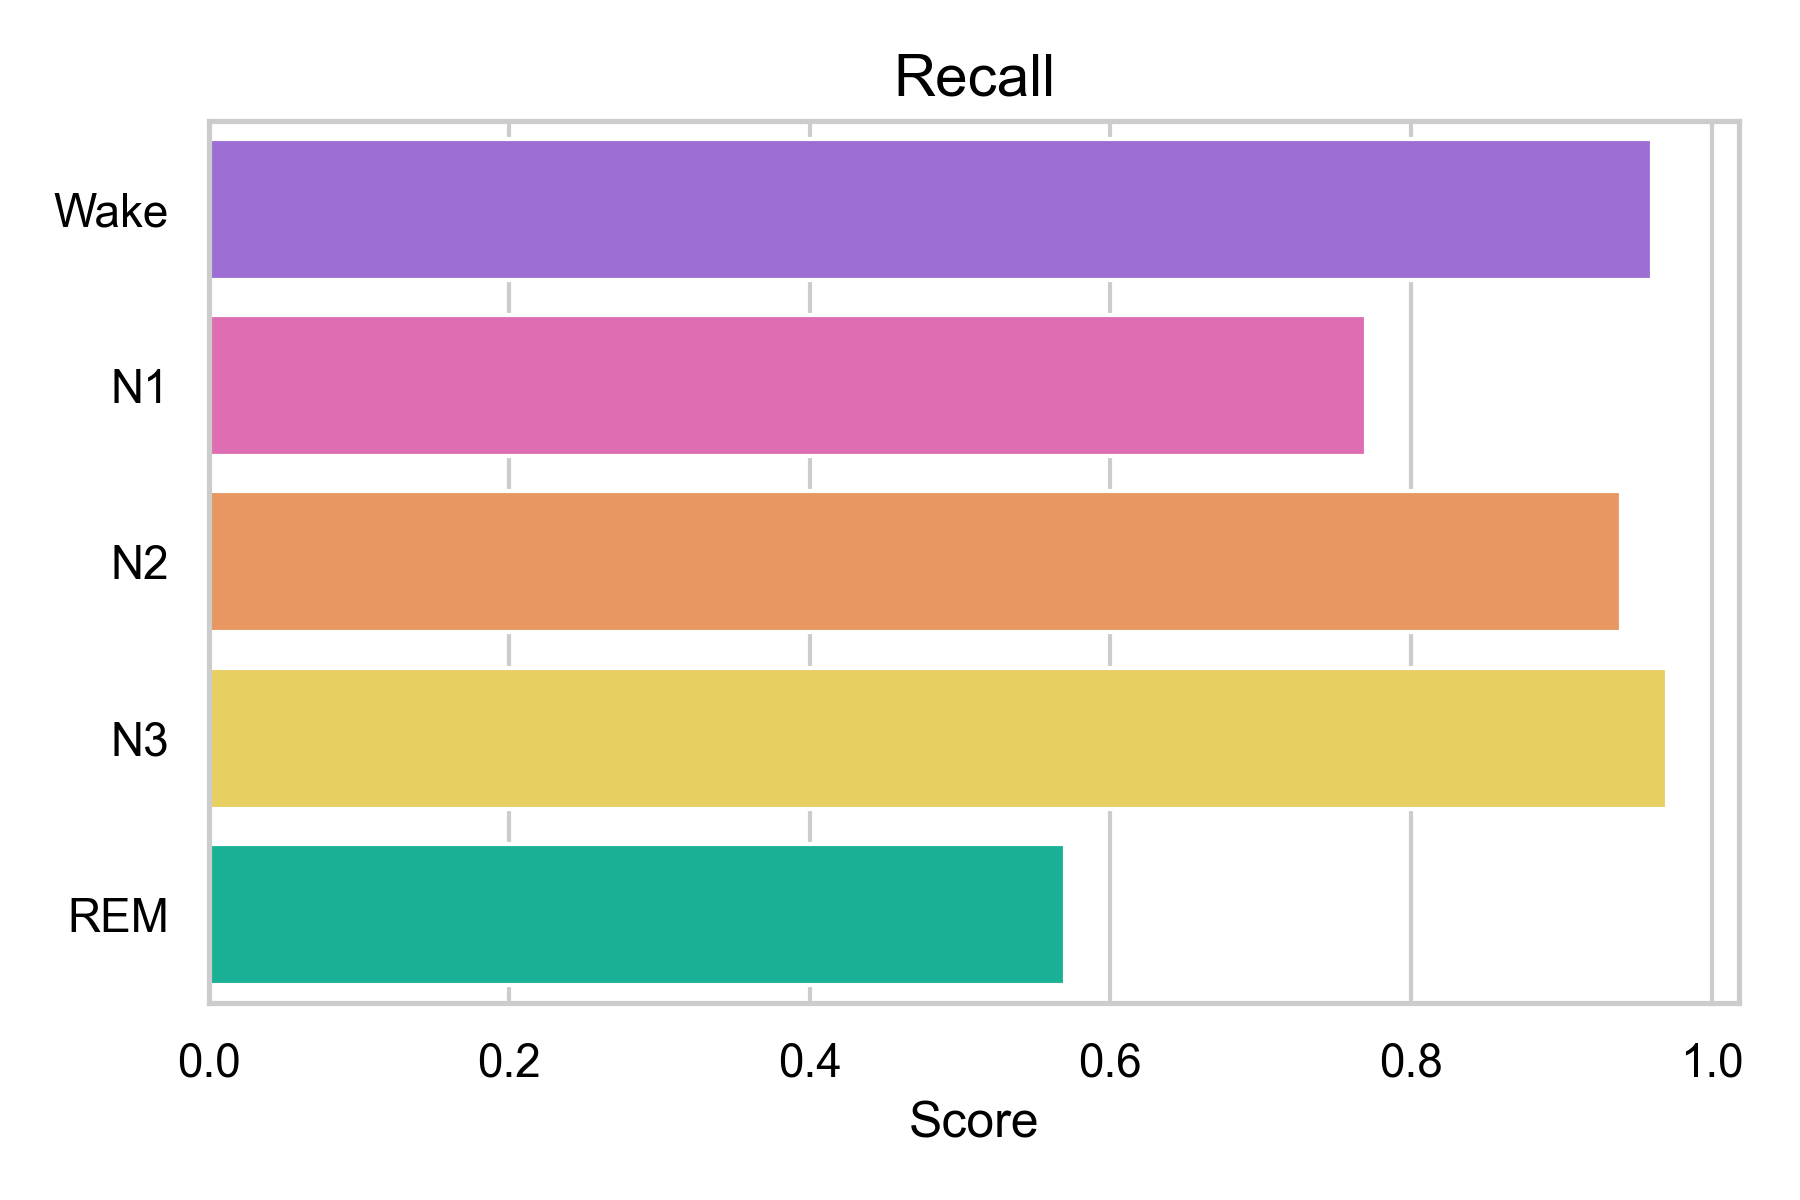
\includegraphics[width=\linewidth]{images/paper_3/recall_plot.png} % Replace with actual figure
        \captionof{figure}{\textcolor{purple}{Recall Scores per Class}}

        % Right Column: F1-Score Bar Plot
        \column{0.33\textwidth}
        \centering
        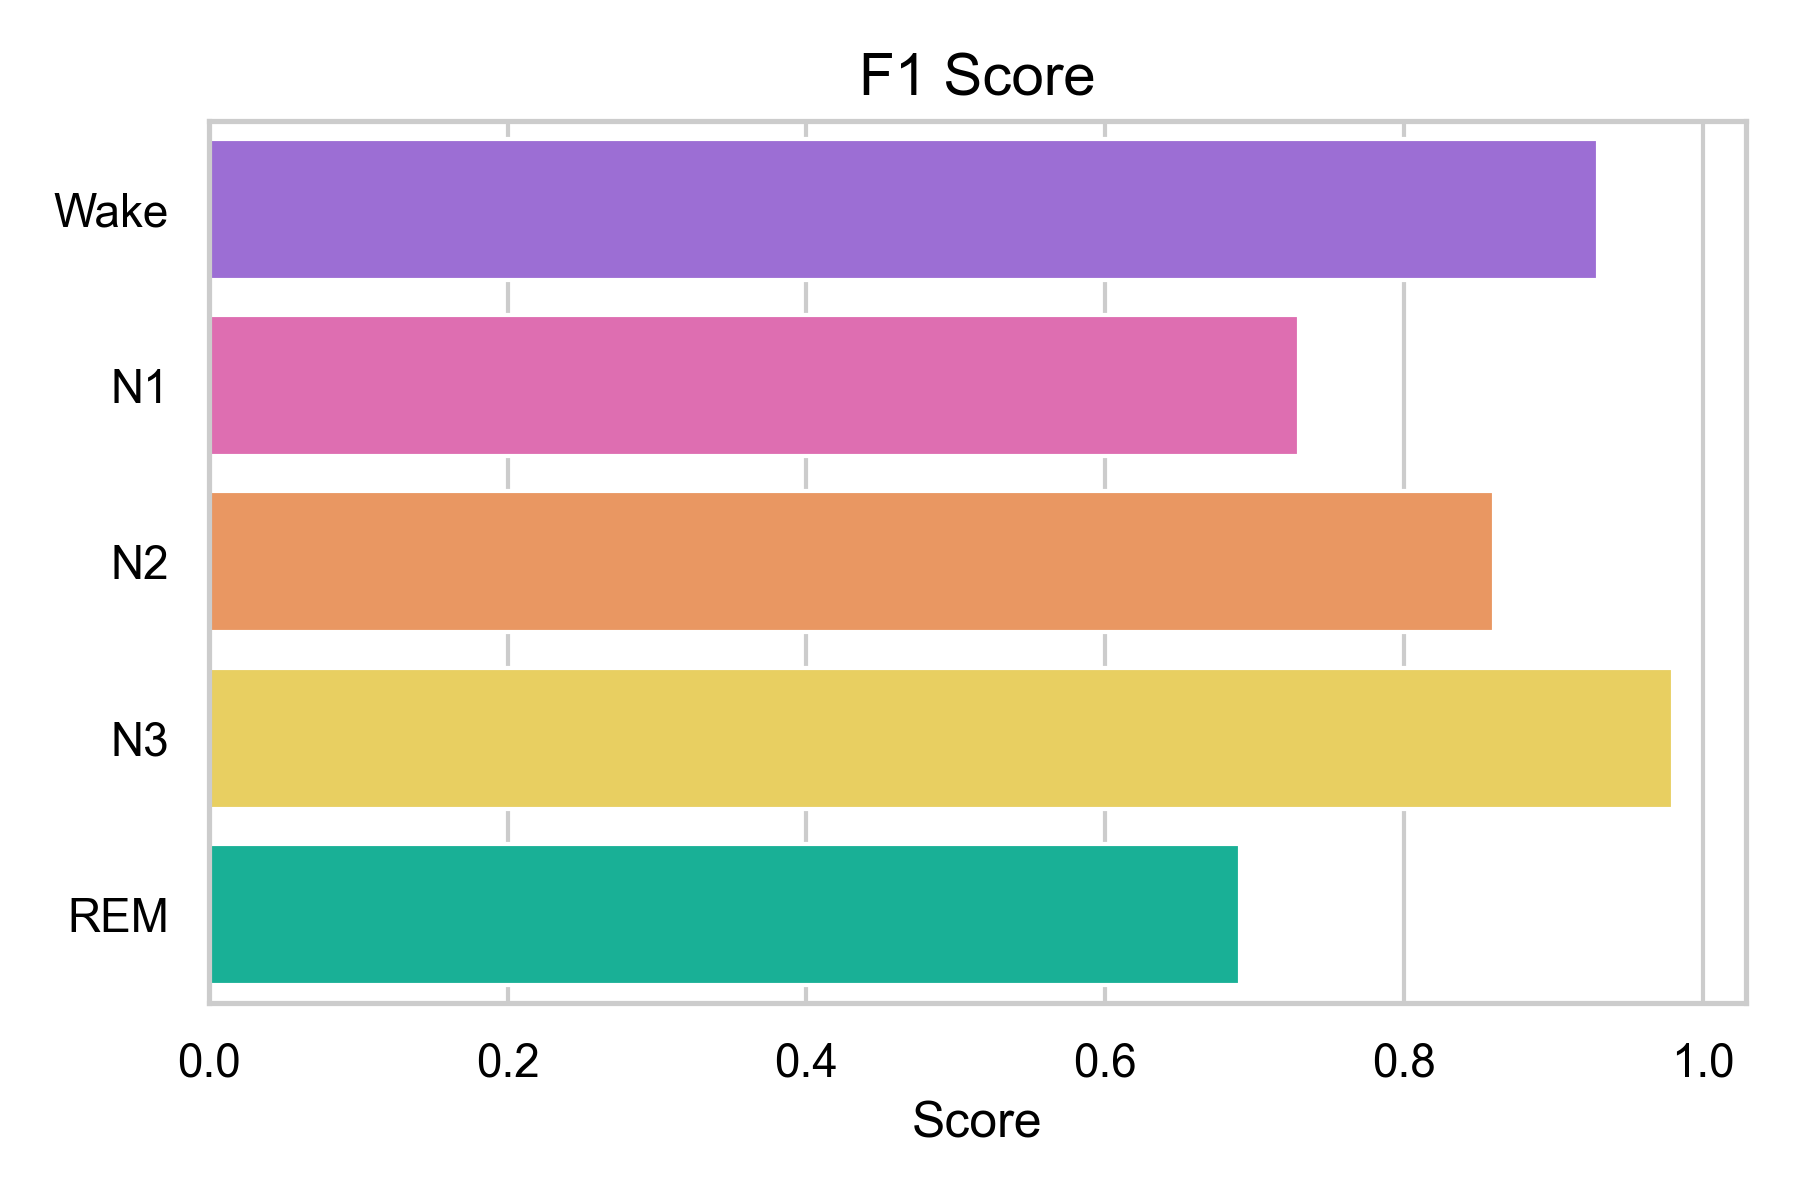
\includegraphics[width=\linewidth]{images/paper_3/f1_score_plot.png} % Replace with actual figure
        \captionof{figure}{\textcolor{purple}{F1 Scores per Class}}
    \end{columns}

\end{frame}

\begin{frame}{Feature Importance Analysis with LIME}

    \begin{columns}

        % Left Column: Explanation
        \column{0.5\textwidth}w
        \textbf{Understanding the contribution of different channels to model predictions.}

        \begin{itemize}
            \item We used \textbf{LIME} (Local Interpretable Model-agnostic Explanations) to analyze feature importance.
            \item The \textbf{EMG submental} and \textbf{EEG Pz-Oz} channels contribute the most to predictions.
            \item \textbf{EOG horizontal} has minimal importance, indicating lower relevance for classification.
            \item This insight helps optimize feature selection and improve model efficiency.
        \end{itemize}

        % Right Column: Figure
        \column{0.5\textwidth}
        \centering
        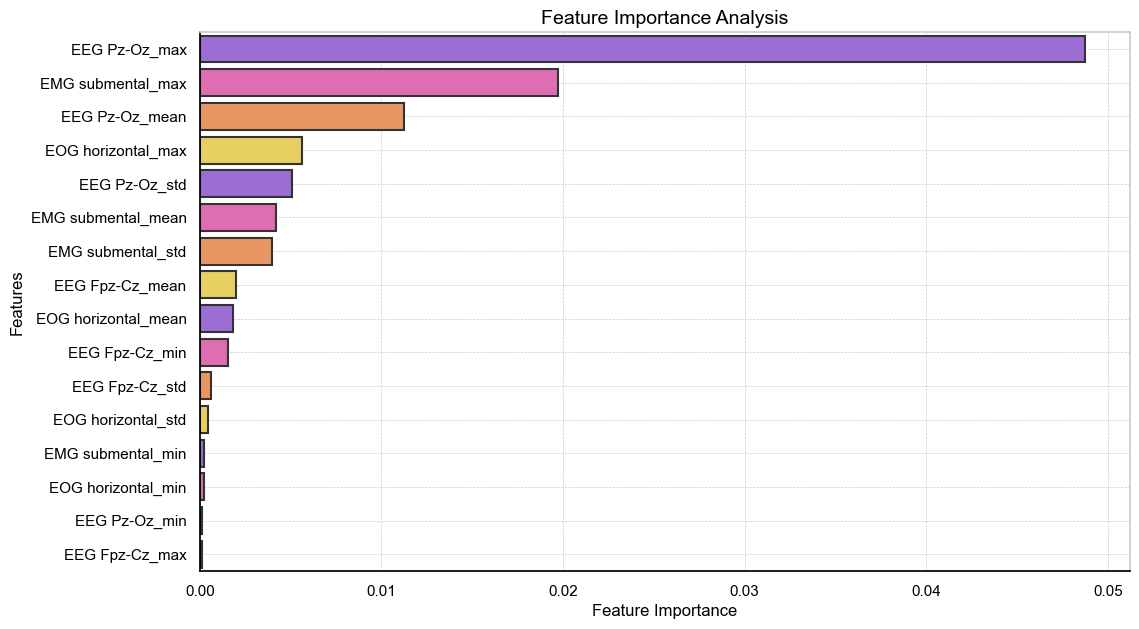
\includegraphics[width=0.9\linewidth]{images/paper_3/feature importance chanels analysis.png} % Replace with actual file path
        \captionof{figure}{\textcolor{purple}{Feature Importance Analysis for 4 Channels}}

    \end{columns}

\end{frame}


